\documentclass{article} % article doctype, possible font size range from 8pt to 20pt with not all being avaiable.
\title{\huge Willy The Robot Advice For Following Groups}
\author{Jeroen van 't Hul\\S1139163  \and Thomas Zwaanswijk\\s1089273 \and Tom van den Noort\\s1101124}
\date{\parbox{\linewidth}{\centering%
	\today\endgraf\bigskip
	Supervisor \hspace*{3cm} Main Stakeholder \endgraf\medskip
	Mischa Mol \hspace*{3cm} Ilja Clabbers \endgraf\bigskip
	Windesheim Zwolle\endgraf}} 


% include packages
\usepackage{graphicx}
\usepackage{caption}
\usepackage{mathabx}
\usepackage{wrapfig}
\usepackage[margin=1.0in]{geometry} % sets page margin, 2.0in is default.
\usepackage{titlesec}
\usepackage{hyperref}
\usepackage[table,xcdraw]{xcolor}
\usepackage{float}
\usepackage[export]{adjustbox}
\usepackage{todonotes}
\usepackage{indentfirst}
\usepackage{blindtext}
\usepackage{scrextend}
\usepackage{textcomp}
%\usepackage{siunitx}
%\usepackage{multirow}	% used for table multirow support
%\usepackage{longtable} % Allows tables to roll over into a new page.
\usepackage[nottoc,numbib]{tocbibind} % Adds bibliography / references to TOC and numbers that section.
\usepackage{array}
\usepackage{footnote}

% ----- custom commands ----- %
% Wrapper for paragraph command. Forces newline after paragraph title
\newcommand{\myparagraph}[1]{\paragraph{#1}\mbox{}\\} % Without \mbox{} all newlines will be ignored, making the first sentence appear on the same line as a paragraph title.
% monospace codeblock
\def\code#1{\texttt{#1}}
% changing the ToC depth in the document enviroment
\newcommand{\changelocaltocdepth}[1]{%
	\addtocontents{toc}{\protect\setcounter{tocdepth}{#1}}%
	\setcounter{tocdepth}{#1}%
}

\newcolumntype{L}[1]{>{\raggedright\let\newline\\\arraybackslash\hspace{0pt}}m{#1}}
\newcolumntype{C}[1]{>{\centering\let\newline\\\arraybackslash\hspace{0pt}}m{#1}}
\newcolumntype{R}[1]{>{\raggedleft\let\newline\\\arraybackslash\hspace{0pt}}m{#1}}

\makesavenoteenv{tabular}
\makesavenoteenv{table}

\setcounter{tocdepth}{2} % only part,chapters,sections, subsections appear in ToC

\addtokomafont{labelinglabel}{\sffamily}

\DeclareCaptionFormat{cancaption}{#1#2#3\par} % Normal format actually
\DeclareCaptionLabelFormat{cancaptionlabel}{#1}
\captionsetup[figure][number]{format=cancaption,labelformat=cancaptionlabel}
\graphicspath { {images/}{../images/} }

\begin{document}
\maketitle

\begin{figure}[H]
\centering
\includegraphics[width=12 cm]{WTRLogo.png}
\end{figure}
\thispagestyle{empty}
\newpage
\setcounter{page}{1}
\tableofcontents
\newpage

% Sections
\section{Introduction}
This research is meant to create an inventory of the current state of the movements WTR\ref{trm::WTR} is capable of performing.
In addition, this document contains a list of proposed improvements in order to increase the accuracy of the autonomous driving.
By creating a list of the range of movement WTR can perform and noting any defects or issues with those, it should become easier to create a proper list of improvements.
Several sections will deal with the sensors, how they benefit the robot and their mounting as well.
\newpage

\section{Product}
\subsection{Current Status of Product}
In the current state, the driving capabilities of WTR have been improved considerably.
The functionality of WTR has been improved through inclusion of an IMU, rotary encoders and the sonar sensors.
While some of these were present at the start of the project, data was either being spoofed or simply not being utilized.

The IMU previously used, the MPU6050, for example was not actually used, and the data was being spoofed so that the robot would move more smoothly.
This has now been corrected, and the actual data received from the new MPU9250 is incorporated into the planning, as well as being more accurate than the old IMU.

The sonars, which previously were not used, are now utilized as well.
Several additional sensors are now located at the back of WTR, so that it can also detect obstacles behind it, so that even during reversing it can be safe.

\subsection{What Could Be Added?}
There are some features that could be implemented in order to increase the safety features of WTR, which are all documented in the separate advice document.
As such, it will not be expanded upon in this document.

\subsection{Schematic Overview}
Figure \ref{fig::schemView} shows the new situation of WTR.
More detailed explanations of every section can be found in the respective documents dealing with those sections.
\begin{figure}[H]
\centering
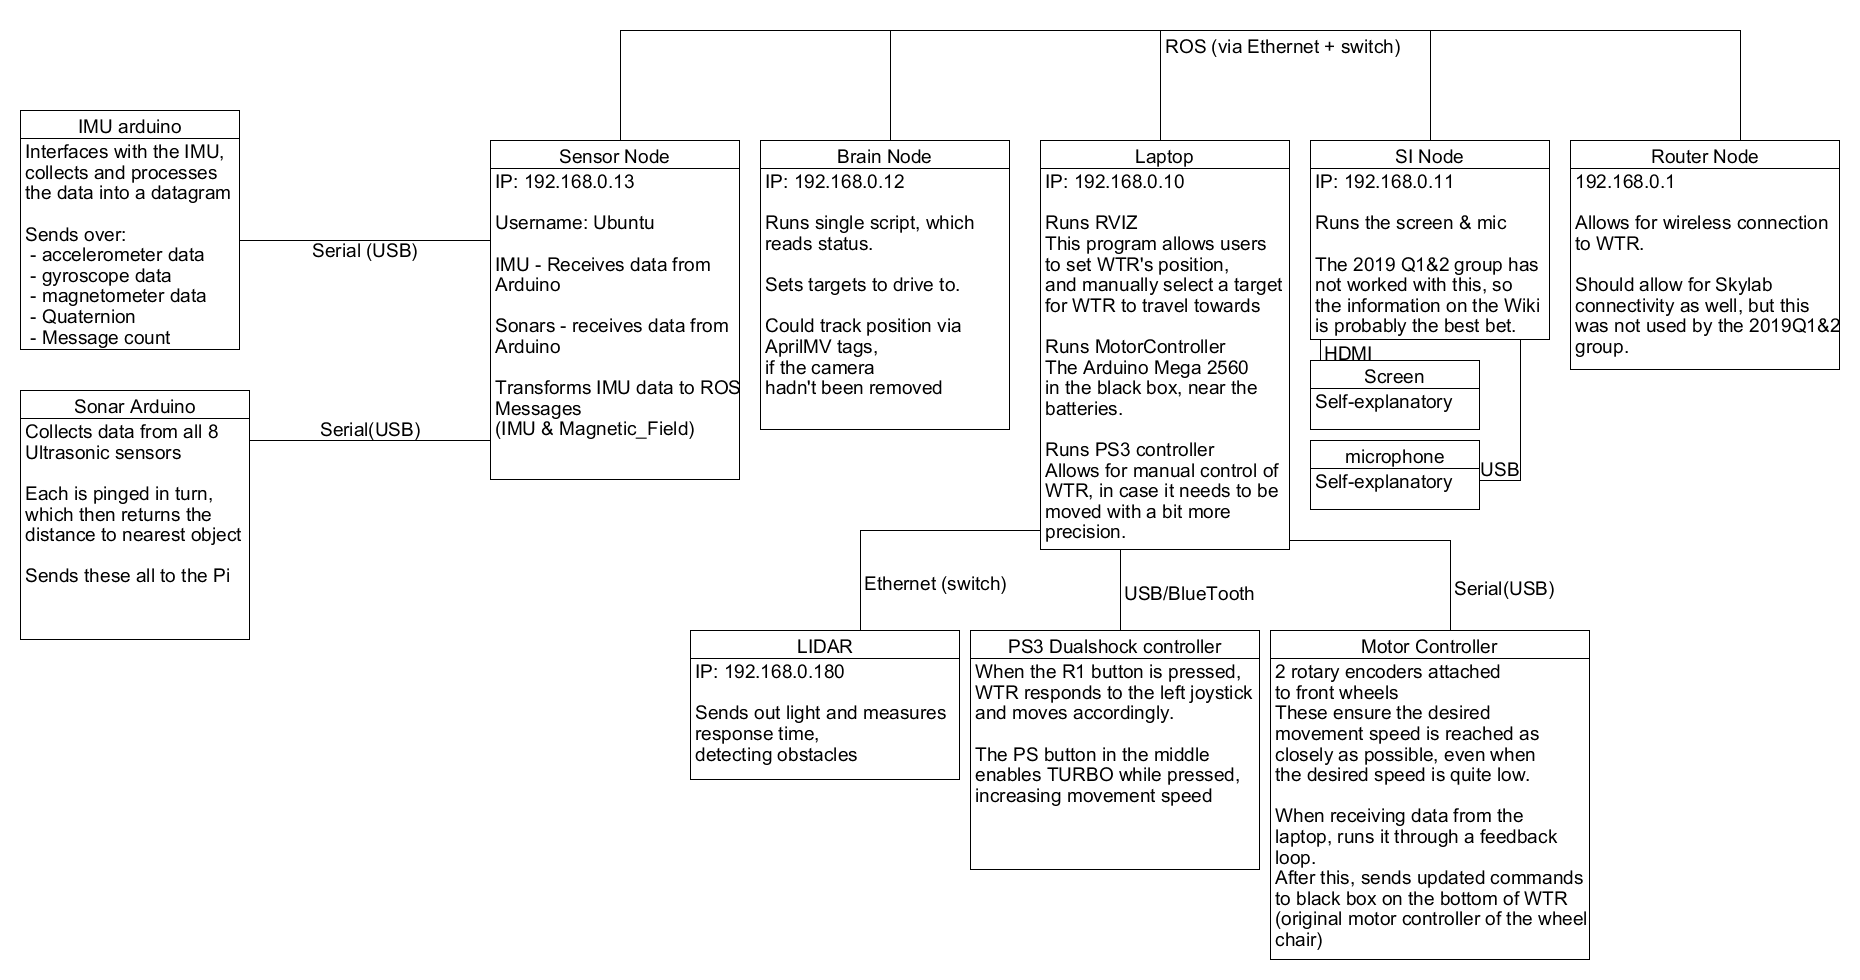
\includegraphics[width=15cm]{rosOverview.png}
\caption{An overview of the separate parts of WTR}
\label{fig::schemView}
\end{figure}

The sensor node communicates with the IMU and the sonar HC-SR04 sensors through arduinos over a serial communication protocol.
This allows easy changes to be made to either section without having to stop both at once, since the node will simply not do anything if it does not receive any messages.

The motor controller is an Arduino Mega 2560, which is connected to the laptop through a USB cable and uses a serial communication protocol as well to translate the commands from RVIZ to a format the P\&G \ref{trm::PGE} can understand and execute.
The feedback loop ensures that it can perform accurately at low velocity as well, rather than blindly sending a speed to it and assuming it is accurate enough to do so.

\newpage

\section{Hardware}
The physical aspect of WTR has massively improved through the use of 3-D printing.
Previously, WTR consisted of a metal frame with wooden planks supporting the laptop and 4 Raspberry Pi's.
This has since been changed to increase the ease of access to every part of WTR.
There are still some parts which need to be updated, however.

\subsection{Batteries}
This group has unfortunately not yet had the chance to fix the battery situation.
While the batteries used are only 24 volt batteries, the idea of having the poles exposed during public expositions and events is not great.
This was something we had planned to correct, but ever got around to.
Some simple caps or covers would be a massive improvement to the current situation.

Another issue that could do with correction is that they are essentially just held in place by weight.
The downside of this is that WTR does not move in what can be described as a smooth fashion.
The robot brakes pretty quickly, so the deceleration is pretty abrupt.
If this happens too often, the batteries could potentially end up touching poles due to the shifting, as the two located under the laptop are on their side.
This could be another issue, but our group did not know enough about electronics to say whether this presented an issue, and as such left it as is.
The advice here is to either cover the poles, again, or create some way of fixing the batteries in place, such as a simple 3-D printed shunt, screwed to the wood.

\subsection{Motor Controller}
The motor controller is located in a black box, in the middle of WTR between several batteries.
While the accessibility has been improved by removing the wooden frame that previously held the laptop and replacing that with a single plank that slots over the frame, it is still not easy to change parts or functionality of the device.
It could be useful, if regular changes are needed, to find a way to move it to a new position, or change the box to not require tape to remain closed.

\subsubsection{Rotary Encoders}
At the time of writing, there is no implemented method of checking whether or not the rotary encoders are still connected.
The risk that comes with this is that the feedback loop model would cause the system to continuously increase the force it outputs until it receives the desired signal.
If the encoders are disconnected, that signal never comes.
This would cause WTR to drive forward at maximum speed the moment it is told to start moving by RVIZ, or the controller.
While the maximum speed is still limited, it will keep attempting to reach it in every motion it makes, especially during turns.
It would be good to implement a method to check for a connection, so that WTR stops when it loses connection to the encoders.

\subsection{TV Screen}
The current TV screen is already a low power model.
However, its current size serves no practical purpose.
Granted, the current group did not have to work with any social interaction, but even if it had been necessary, this screen would be considered overkill.
The next group should consider changing to a smaller screen, if only for testing purposes.
The size of the screen causes it to drain the battery quicker, so a small screen would allow for more rigorous testing.

The 2018 Q3\&Q4 group recommended a touch screen, and this group supports that decision.
A smaller touch screen allows for a longer battery life, while simultaneously increasing the options for interacting with WTR.

\subsection{Laptop}
The laptop currently runs on its own battery, which is \textit{theoretically} fine.
It is capable of running RVIZ, and communicating with all the nodes.
The downside of it running on a separate battery is that it does drain rather quickly.
A simple trip from the innovation lab on T5 to the printer located on the other side of the bridge between the two sides of the building can drain the battery by as much as 50 percent, which is not desirable.
In cupboard C, there is a transformer which could be attached to the batteries that allows the laptop charger to be plugged into it and power the laptop.
The 2019 Q1\&Q2 group did not attach it, because the testing that was done did not require WTR to drive very far from the innovation lab.
If more extensive testing is planned, this might be considered a smart move.

\subsection{IMU}
The IMU \ref{trm::imu} is located on top of the screen, as magnetic interference caused by the electrical motors and the steel frame would otherwise prevent the magnetometer from operating properly.
It has been clipped there using a 3-D printed box, but during the design of that a few dimensions of the TV screen were forgotten, causing the IMU to be slightly misaligned.
While this does not cause any major issues, the slightly inaccuracy in the design prevents the IMU from being as snugly fitted to the screen, allowing it to shake around a bit.
A more tightly designed container would help increase the stability of the readings.

\newpage

\section{Software}
No project in an IT minor could be complete without a considerable amount of software.
The 2019 Q1\&Q2 team made a few a mistakes in handling it, which caused avoidable issues.

\subsection{GitHub}
The team made their own repository for their code, which meant that there was a more complex merging process than was exactly necessary.
Instead, consider forking the existing \href{https://github.com/Windesheim-Willy/}{repo}, so that the merging process can happen as a standard git pull request.

\subsection{ROS}
There are a lot of complexities to ROS, or Robotic Operating System.
The first is that it is not exactly an operating system.
It functions more akin to a bus that allows publishing and subscribing to topics.
The mistake made by the group here was that we fundamentally misunderstood this for the first few weeks, and as such wasted time in how the system was changed.

\subsubsection{Control Panel}
The program used to plan the route WTR will take to a goal, as well as the system to set a goal, is called RVIZ.
This can be accessed by using the command "startwilly" in a terminal on the laptop.
The group attempted to make this an easier task, by creating a control panel to reduce this to a simple button press.
The unfortunate side of this was that due to the way Python created and killed of tasks, memory leaks caused the laptop to crash if it ran for too long.
The concept itself is a very good idea, though.
By creating a simple program that can be started up on boot, which allows users to activate or stop certain parts of WTR can mean that troubleshooting can be made much easier, as well as creating a simpler start-up process.

\subsubsection{RVIZ and Plugins}
In order to integrate all the different methods of tracking orientation and obstacles, many RVIZ plugins were installed.
It is worth reading up on these before editing variables or configuration files, as many of these have rather obfuscated names.
An example of this can be found in the \code{RQTconfig} system, where several variables are named along the lines of \code{Alpha\_1}, or \code{Alpha\_2}.
Most plugins conform to the ROS REP standards, which are also worth checking out, especially \href{https://www.ros.org/reps/rep-0103.html}{103}  and \href{https://www.ros.org/reps/rep-0105.html}{105}, which deal with the units data are measured in and the coordinate systems used in mobile platforms, respectively.
If these standards are not conformed to, ROS and RVIZ will start producing errors.

\newpage
\section{Security}
There are essentially two aspects to the security of WTR.
The first is the risk a malicious third party could pose to WTR if they wanted to abuse it.
The second is the risk WTR poses to the world around it.

\subsection{Vulnerabilities}
Ideally, WTR should be an air-gapped robot, with no possibility of wireless access, since it is going to be driving around at public events.
If WTR is broadcasting a network, then it would be possible to enter that and start commanding WTR to drive into people, for example.
Since this is unfortunately not possible as several social interaction features require an internet connection to some degree.

The likelihood of someone wanting to abuse WTR is quite small.
It has no connection to the network at the time of writing, and does not track any personal data.
There is essentially nothing of value to be gained by hacking WTR, so if it was done, it would most likely happen for the sake of a joke or prestige.
It would not exactly be difficult to hack either, due to the standardized nature of ROS.
ROS has set formats for every message, so a spoofed message to the \code{cmd\_vel} topic could cause WTR to over-accelerate, or drive straight into a wall.

Another vulnerability is that if someone has physical access to the switch, they could start spoofing messages and causing WTR to either crash or start behaving anomalously.
In order to prevent this, a small cover or physical protection could be used, such as a plexiglass cover that allows the internals of WTR to remain visible while preventing undesired physical access.

It would be advisable, however, to ensure that WTR gets an upgrade to its passwords.
Unfortunately, this group did not have the time to do this, but many of the passwords are vulnerable to botnets or other malicious attacks that exploit default passwords.
Many passwords are very weak, and could do with some updates.

\subsection{Danger to Others}
At the moment, WTR is a lot less dangerous to the world around it than it was at the start of the project.
Previously, it had several sharp edges that ended up costing a member of the team a pair of jeans, so the issue had to be taken care of.

Since then, it has had covers placed over all sharp edges that could hit someone while WTR is moving.
There are still some sharp bits, but due to a lack of angle grinder this group was unable to fix this.

The batteries are still only kept in place due to their weight, so a sudden stop due to a collision or abrupt stop signal could shift the batteries, potentially snapping cables or such.
As is noted in the advice document, this needs updating.
Another point mentioned is the exposed parts, which while not life-threatening as the batteries only run at 24 volt, are still not exactly good to have exposed.
Again, refer to the advice document for the group opinion on how to solve these issues.

\newpage

\section{Knowledge}
Since ROS is a very academically focussed system, a lot of knowledge is shared online.
When the group ran into issues and went to the ROS version of stackoverflow, \href{https://answers.ros.org/questions/}{ROS answers}, any questions asked generally received an answer very quickly.
This is worth checking out if anyone gets stuck trying to integrate new functionality in the system, or is confused about how certain parts are implemented.

\todo{Tom/jeroen, mss hier nog wat schrijven?}
\section{Advice to the Product Owner}
Naturally, aside from advice to the following groups, there is also some feedback to the product owner.

\subsection{Future Technology}
As a part of the future technology, it is expected that the technology is somewhat experimental.
Unfortunately, the system used here is actually starting to become rather antiquated.
The developers of ROS have already released working versions of its successor, ROS 2.
Another issue is that ROS 1 currently runs on Ubuntu 16.0.4, while at the time of writing, Ubuntu has released version 19 already.
It could be worth asking a following group that works on the project to attempt to update any possible sections to those newer versions, since support for the current systems is likely to be dropped.

\subsection{Ask For a Clear Inventory of Capabilities}
More than once the current group ran into a bit of a sticking point when discussing what the target for WTR would be as a project.
The goal that was set at the start was rather nebulous,  "Improve WTR's driving capabilities".
This did not present a clear goal, though it was later refined a fair bit.
The issue with the new goal, which was communicated to the group halfway through the project, was that it did not line up with the capabilities of WTR.
The goal to have WTR drive at a person when it recognized one was unrealistic, since the way WTR deals with facial recognition is not usable in navigation.
The summary of this advice would be to take a critical look at its functionality, and determine ahead of time what the goal would be so that it is possible for the group to work towards the same goal with a clear target in mind.
In order to do this, create an inventory of current capabilities, such as driving to a pre-determined place, creating a new goal on the fly, or to track a human face in a better way than WTR currently does.

\subsection{Social Interaction}
As was mentioned in the introduction of this document \ref{sec::intro}, the only real problem area left for WTR is social interaction.
The 2019 Q1\&Q2 group did not investigate this much, as it laid outside of our project scope, but from the casual investigation into the related capabilities, it became obvious that there is still room for improvement.

\subsubsection{Boxes and Cupboards}
While testing WTR, on startup it also launches its webcam and facial recognition software.
It was greatly amusing to the group to find out what WTR considers a face.
Among those options are:
\begin{itemize}
\item Cardboard boxes
\item Whiteboards
\item The racks for the first KBS (the ASRS system)
\item empty space
\item windows
\item chairs
\end{itemize}
Facial recognition is of course a very complicated section of programming, as properly tracking several hundreds of faces is something the entire government of China has only recently achieved.


\appendix  %all sections after this are appendices
\section{Glossary}
\begin{itemize}
\item \label{trm::dms} Dead-man's switch - a button on a controlling unit which has to be held down in order to have the robot respond to inputs. This is generally done in order ensure a machine cannot perform any actions should the controller be dropped or receive inputs without proper supervision.
\item WTR - Willy The Robot.
\end{itemize}
\newpage
\bibliographystyle{ieeetr}
\bibliography{references}



\end{document}
